\chapter{Fortgeschrittene Synchronisationskonzepte in Java}


\section{Semaphore}

Der \textbf{Semaphor} (engl. ``semaphore``) repräsentiert ein klassisches Synchronisationskonzept.\\

\noindent
Das abstrakte Konzept dahinter: Ein Semaphor hat einen Wert des Typs \code{int}, der nie $<\ 0$ werden kann.\\
Die Methoden \code{p()} (nl.: \textit{passeeren}, auch engl. \textit{down} oder \textit{acquire}) bzw. \code{v()} (nl. \textit{frijgeven}, auch engl. \textit{up} oder \textit{release}) dienen zum Herunter- bzw. Hochzählen des Attributs.\\

\noindent
Ein Thread wird \textbf{blockiert}, wenn bei seinem Aufruf von \code{p()} der Attributwert negativ werden würde.

\subsection{Einfache Semaphore für den gegenseitigen Ausschluss}

Semaphoren werden häufig zur Realisierung des gegenseitigen Ausschlusses realisiert $\rightarrow$ ein Programmstück kann nur von einem Thread gleichzeitig ausgeführt werden.\\

\noindent
Hierzu werden sogenannte \textbf{Mutex Semaphors} (\textit{Mutex} = \textit{Mutual Exclusion}) verwendet:\\
Die Semaphor wird hierzu mit dem Wert $1$ initialisiert - ruft ein Thread $t_1$ \code{p()} auf und zählt dabei den Wert des Semaphors herunter, müssen ankommende Threads $t$ warten, bis der Wert durch die Freigabe von $t_1$ wieder erhöht und so der kritische Bereich\footnote{
    \textit{kritischer Bereich}: das Programmstück, das zu einem Zeitpunkt nur von höchstens einem Thread ausgeführt werden darf (vgl.~\cite[102]{Oec22}).
} wieder freigegeben wird\footnote{eine \textit{binäre Semaphore} kann nur die Werte $0$ und $1$ bzw. $true$ und $false$ annehmen. In \textit{v()} kann vor dem \textit{notify} überprüft werden, ob sich die Semaphore gerade überhaupt im ``gesperrten`` Zustand befindet}.\\

\noindent
In dem folgenden Beispiel wird \underlien{ein} Semaphor für 3 verschiedene Objekte desselben Typs verwendet.\\
Der Semaphor stellt sicher, dass nur jeweils ein Thread das Programmstück in \code{enter()} (über die $3$ verschiedenen Objekte verteilt) ausführen kann. \\


\begin{minted}[mathescape,
    linenos,
    numbersep=5pt,
    gobble=2,
    fontsize=\small,
    frame=lines,
    framesep=2mm]{java}
    public class MutexSemaphorDemo {

        static class MutexSemaphor {
            private int n = 1;
            public synchronized void p() {
                while (n < 1) {
                    try {
                        wait();
                    } catch (InterruptedException ignored) {}
                }
                n--;
            }

            public synchronized void v() {
                n++;
                notify();
            }
        }

        static class Waiter extends Thread{
            MutexSemaphor sem;
            String name;
            public Waiter(MutexSemaphor s, String n) {
                sem = s;
                name = n;
                start();
            }

            public void enter() {
                    String currentThread = Thread.currentThread().getName();
                    sem.p();
                    System.out.println(currentThread + " enters [" + name + "]!");
                    try {
                        Thread.currentThread().sleep((int) (Math.random() * 100));
                    } catch (InterruptedException ignored) {}
                    System.out.println(currentThread + " exits [" + name + "]");
                    sem.v();
            }
        }

        public static void main(String[] args) throws InterruptedException {
            MutexSemaphor sem = new MutexSemaphor();
            Waiter waiter1 = new Waiter(sem, "w1");
            Waiter waiter2 = new Waiter(sem, "w2");
            Waiter waiter3 = new Waiter(sem, "w3");
            Thread t1 = new Thread(waiter1::enter);
            Thread t2 = new Thread(waiter2::enter);
            Thread t3 = new Thread(waiter3::enter);

            t1.start();t2.start();t3.start();
            t1.join();t2.join();t3.join();
        }
    }
\end{minted}\\

Eine mögliche Ausgabe für das Programm ist:\\

\noindent
\begin{minted}[mathescape,
    numbersep=5pt,
    gobble=2,
    frame=lines,
    framesep=2mm]{bash}
    Thread-3 enters critical section of [w1]!
    Thread-3 exits [w1]
    Thread-4 enters critical section of [w2]!
    Thread-4 exits [w2]
    Thread-5 enters critical section of [w3]!
    Thread-5 exits [w3]
\end{minted}\\

\noindent
Wäre \code{enter} hingegen bloß \code{synchronized} und es würde kein Semaphor verwendet, würden die Threads jeweils parallel \code{enter} ausführen, die Ausgabe lautet dann in etwa:


\begin{minted}[mathescape,
    numbersep=5pt,
    gobble=2,
    frame=lines,
    framesep=2mm]{bash}
    Thread-3 enters critical section of [w1]!
    Thread-4 enters critical section of [w2]!
    Thread-5 enters critical section of [w3]!
    Thread-4 exits [w2]
    Thread-3 exits [w1]
    Thread-5 exits [w3]
\end{minted}\\

\subsection{Semaphore zur Herstellung vorgegebener Ausführungsreihenfolgen}

Neben gegenseitigem Ausschluss können Semaphoren auch eingesetzt werden, um die \textbf{Ausführungsreihenfolge} von Threads festzulegen\footnote{ausführliches Beispiel in~\cite[104]{Oec22}}.

\subsection{Additive Semaphore}
\textbf{Additive Semaphore} erlauben es aufrufenden Threads, den Wert einer Semaphore um ein gewisses $\Delta\ (\geq\ 1)$ herunterzuzählen.\\

\noindent
Dabei ändert sich die Wartebedingung in des Semaphors von

\begin{minted}[mathescape,
    linenos,
    numbersep=5pt,
    gobble=2,
    frame=lines,
    framesep=2mm]{java}
    while (n == 0) {
        //...
    }
\end{minted}\\

zu

\begin{minted}[mathescape,
    linenos,
    numbersep=5pt,
    gobble=2,
    frame=lines,
    framesep=2mm]{java}
    while (n - x < 0) {
        //...
    }
\end{minted}\\

\noindent
Durch die parametrisierte Wertebedingung ist es nötig, wartende Threads mittels \code{notifyAll()} aus der Warteschlange zu holen: Erstens kann es mehrere Threads geben, bei denen insgesamt $\sum_{i=1}^{n} \Delta_i\ \geq\ 0$ sein kann (es dürfen dann mehrere Threads parallel in den kritischen Bereich); zweitens kann die Wartebedingung basierend auf dem $x$ für Threads unterschiedlich sein - sollte nur \code{notify} verwendet werden kann es passieren, dass ein Thread direkt danach wieder in die Warteschlange kommt - und infolgedessen kein anderer Thread mehr in den kritischen Bereich, und kein Aufruf von \code{v()} mehr stattfindet.\\

\indent
Selbstverständlich sollte sein, dass der Wert des Semaphors \textbf{auf einen Schlag} (durch Subtraktion / Addition) verändert wird, ansonsten kann es zu einer \textbf{Verklemmungssituation} kommen, wenn der Wert inkrementiert/dekrementiert wird (vgl.~\cite[109]{Oec22}).

\subsection{Semaphorgruppen}

Die grundlegende Eigenschaft von additiven Semaphoren, den Wert eines Semaphores auf einen Schlag zu ändern, ist Motivation für die Einführung von \textbf{Semaphorgruppen}.\\

\noindent
Semaphorgruppen werden nicht als Felder von Semaphoren angelegt, sondern eine Semaphorgruppe enthält ein Feld von Werten, auf dem operiert wird.\\

\noindent
Jeder Eintrag in dem Feld repräsentiert ein Mitglied der Semaphorgruppe.


\noindent
Auf die Implementierung von \code{p()}/\code{v()} wird hierbei verzichtet - stattdessen gibt es eine Methode mit einer Signatur ähnlich zu

\begin{minted}[mathescape,
    numbersep=5pt,
    gobble=2,
    frame=none,
    framesep=2mm]{java}
    public synchronized void changeValues(int[] deltas)
\end{minted}\\

\noindent
Die Methode schiebt so lange einen Thread in eine Warteschlange, bis die Wartebedingung nicht mehr erfüllt ist - hierbei wird dann jeder Index von der Semaphore wie folgt überprüft:


\begin{minted}[mathescape,
    numbersep=5pt,
    gobble=2,
    frame=none,
    framesep=2mm]{java}
    if (values[i] + delta[i] < 0) {
        return false
    }
\end{minted}\\

Änderungen werden dann nur durchgeführt, wenn nach der Änderung die Werte aller Semaphore der Gruppe nicht negativ sind (vgl.~\cite[109]{Oec22}).\\

\noindent
Wie bei der additiven Semaphore ist es nötig, Threads über \code{notifyAll()} aus der Warteschlange zu holen - ansonsten kann es auch hier vorkommen, dass ein Thread, der weiterlaufen könnte, nicht geweckt wird.\\

\noindent
Das folgende Beispiel zeigt eine Implementierung einer einfachen Semaphorgruppe (vgl.~\cite[110, Listing 3.5]{Oec22} .
Auf die Überprüfung der Argumente in den Methoden (Eingabelänge == Argumentlänge) wurde verzichtet.

\begin{minted}[mathescape,
    linenos,
    numbersep=5pt,
    gobble=2,
    fontsize=\small,
    frame=lines,
    framesep=2mm]{java}
    class SemaphoreGroup {
        int[] values;
        public SemaphoreGroup (int n) {
            values = new int[n];
            for (int i = 0; i < n; i++) {
                values[i] = 1;
            }
        }

        public synchronized void change(int[] set) {

            while (!canChange(set)) {
                try {
                    wait();
                } catch (InterruptedException ignored) {}
            }

            changeValues(set);
            notifyAll();
        }

        private void changeValues(int[] set) {
            for (int i = 0; i < set.length; i++) {
                values[i] =  values[i] + set[i];
            }
        }

        private boolean canChange(int[] set) {
            for (int i = 0; i < set.length; i++) {
                if (values[i] + set[i] < 0) {
                    return false;
                }
            }
            return true;
        }

    }
\end{minted}



\subsection{Notizen zu den Übungen}

Die Abfrage von Außen auf Listen/Felder von Threads, die sich derzeitig in der Warteschlange befinden, sollte \code{synchronized} erfolgen.
Außerdem sollte eine Kopie der Listen zurückgegeben werden, um Manipulation an der tatsächlichen Liste zu verhindern.\\

\noindent
Bei Exceptions, die nicht abgefangen werden, sorgt \code{finally} für ein Ausführen des durch \textit{finally} eingeleiteten Anweisungsblock auch im Fall einer Exception\footnote{
Java Language Specification - 14.20.2. Execution of try-finally and try-catch-finally : \url{https://docs.oracle.com/javase/specs/jls/se21/html/jls-14.html#jls-14.20.2} - abgerufen 26.01.2024
}, wie folgendes Beispiel zeigt:

\newpage
\begin{minted}[mathescape,
    linenos,
    numbersep=5pt,
    gobble=2,
    fontsize=\small,
    frame=lines,
    framesep=2mm]{java}
    public class TryCatchDemo {

        public String m1(boolean exc) {
            try {

                System.out.println("try 1.");

                if (exc) {
                    throw new Exception();
                }
                System.out.println("try 2.");

                return "foo";

            } catch (Exception e) {

                return "Exception.";

            } finally {
                System.out.println("finally.");
            }
        }

        public static void main(String[] args) {
           TryCatchDemo demo = new TryCatchDemo();
           System.out.println(demo.m1(false));
           System.out.println();
           System.out.println(demo.m1(true));
        }

    }
\end{minted}\\

Die Ausgabe des Programms lautet:


\noindent
\begin{minted}[mathescape,
    numbersep=5pt,
    gobble=2,
    frame=lines,
    framesep=2mm]{bash}
    try 1.
    try 2.
    finally.
    foo

    try 1.
    finally.
    Exception.
\end{minted}\\


\section{Message Queues}\label{sec:messagequeues}

\subsection{Verallgemeinerung des Erzeuger-Verbraucher-Problems}

Bei \textbf{Message Queues} bleiben Nachrichten als Einheiten erhalten (\textbf{nachrichtenorientierte Kommunikation}, bspw. \textbf{UDP}\footnote{User Datagram Protocol}).\\

\noindent
\textbf{Pipes} repräsentieren \textbf{datenstromorientierte Kommunikationsmodelle} (bspw. \textbf{TCP}\footnote{Transmission Control Protocol})  - der Empfänger sieht nicht, in welchen Portionen die Daten gesendet werden.\\

\noindent
Eine Message Queue besitzt einen \textbf{Puffer}, der entweder viele kleine oder wenig große Nachrichten entgegennehmen kann.\\

\noindent
Bei \textbf{Message Queues} werden die Nachrichten in ihrer Gesamtheit in Feldern gespeichert (bspw.~\code{byte[][]}).\\

\noindent
Bei \textbf{Pipes} werden Nachrichten in eindimensionalen Feldern (bspw.~\code{byte[]}) gespeichert (in zyklischer Weise) - dadurch sind Nachrichtengrenzen nicht zu erkennen.\\

\noindent
Das Senden bei Pipes erfolgt i.d.R. als unteilbare Aktion.
\begin{itemize}
    \item Wenn die Nachricht größer ist als der \underline{im Puffer verbleibende Platz}, wird gewartet, bis der Platz frei ist - dann wird \textbf{auf einen Schlag} in den Puffer kopiert
    \item Ist die Nachricht länger als \underline{die Größe des Puffers}, wird die Nachricht geteilt und in Portionen gesendet - dadurch kann es vorkommen, dass Nachrichtenteile durchgemischt werden; sind die Nachrichtenteile nicht größer als die Pufferlänge, befinden sie sich komplett im Puffer;  umgekehrt ist es möglich, dass Stücke von Nachrichtenteilen ``durchgemischt`` werden (vgl.~\cite[117 f.]{Oec22}).
\end{itemize}

Beim Empfangen wird nur so lange gewartet, bis der Puffer nicht mehr leer ist:
\begin{itemize}
    \item der Empfänger gibt an, wie viele Bytes ($n$) er lesen möchte.
    \item ist der Puffer komplett leer, wird mit dem Lesen gewartet, bis Daten im Puffer sind.
    \item Es werden $n$ Daten aus dem Puffer gelesen - sind weniger als $n$ Daten im Puffer, werden auch nur soviele Daten gelesen (die Daten werden hierbei in ein Feld passender Länge kopiert).
\end{itemize}

\section{Das Philosophen-Problem}
 Das \textbf{Philosophen-Problem}\footnote{
Wikipedia - Dining Philosophers Problem: \url{https://en.wikipedia.org/wiki/Dining_philosophers_problem} - abgerufen 27.01.2024
}
veranschaulicht die Entstehung von Verklemmungen: An einem runden Tisch sitzen 5 Philosophen ($P_1,...,P_5$), die abwechselnd mit Denken und Essen beschäftigt sind.\\

\begin{figure}
    \centering
    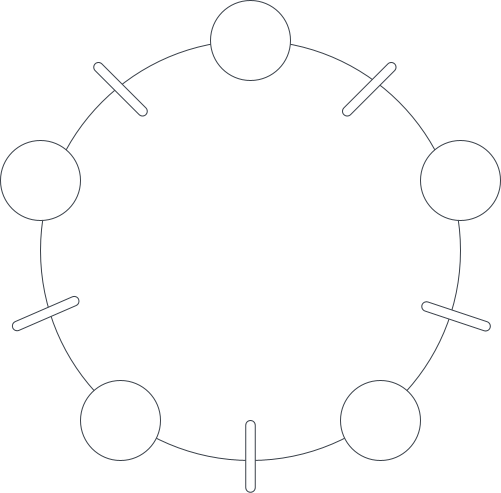
\includegraphics[scale=0.25]{chapters/3/img/philosopher}
    \caption{ Eine Illustration des Philosophen-Problems: Ein Philosoph benötigt jeweils die Gabel links und rechts von ihm zum Essen (Quelle: eigene)}
    \label{fig:philosopher}
\end{figure}


 Zum Essen benötigen die Philosophen Gabeln, und zwar eine in jeder Hand.
 Die Gabeln liegen genau zwischen den Philosophen.
 Angenommen, alle Philosophen sind mit Denken beschäftigt.
 Wenn jetzt ein Philosoph $P_1$ davon zum Essen übergeht, greift er links eine Gabel, und genau in dem Moment wollen die anderen Philosophen auch zum Essen übergehen: Alle nehmen ihre linken Gabeln.
$P_1$ möchte nun die rechte Gabel nehmen, die aber als linke Gabel von $P_5$ von diesem gehalten wird - also muss $P_1$ warten, bis $P_5$ seine Gabel freigibt - der gleichzeitig aber nicht essen kann, weil er dazu die Gabel benötigt, die $P_4$ hält.
Da alle Philosophen auf eine Freigabe der Gabeln warten, kommt keiner dazu, zu essen.\\

\noindent
Diese Verklemmungssituation läßt sich bspw. durch Semaphorgruppen lösen, wobei ein Philosoph jeweils zwei Gabeln \textbf{auf einen Schlag} anfordert, oder auch durch $n$ Semaphoren, wobei jeder Semaphor eine Gabel repräsentiert, und ein zusätzlicher Semaphor als ``Essenserlaubnis``, die den ``Gabel-Semaphoren`` vorgeschaltet ist, wie im folgenden Beispiel:

\begin{minted}[mathescape,
    linenos,
    numbersep=5pt,
    gobble=2,
    fontsize=\small,
    frame=lines,
    framesep=2mm]{java}
    public void run() {
        while (true) {
            // eatLock ist eine Mutex-Semaphore.
            // left() und right() rufen jeweils p()
            // (bzw. v() wenn release == true) auf
            // die benachbarten Gabeln auf (wobei Gabel rechts ==
            // index des aufrufenden Philosophen ist)
            eatLock.acquire();
            table.left(position, false).right(position, false);
            eatLock.release();

            table.left(position, true).right(position, true);
        }
\end{minted}\\



\section{Leser-Schreiber-Problem}

\textbf{Leser-Schreiber-Problem}: Es soll lesen erlaubt sein von beliebig vielen Threads, aber die Änderung des Objekts durch schreibende Zugriffe darf nur von einem Thread aus geschehen.\\

\noindent
Wenn alle Zugriffe \textbf{synchron} sein müssen, würde das Objekt beim Lesen als auch beim Schreiben blockiert - das schränkt die Parallelität ein, vor allem, wenn der Lesevorgang länger dauert und das Objekt somit nicht aktualisiert werden kann.\\

\noindent
$\rightarrow$ Es muss eine Lösung gefunden werden, so dass mehrere Threads lesen, aber nur ein Thread schreiben kann.

Zur Lösung sind verschiedene Strategien denkbar:

\begin{itemize}
    \item Bevorzugung der Leser, falls es darauf ankommt, dass die Leser schnell Zugriff auf die Daten erhalten, und die Aktualität der Daten weniger wichtig ist
    \item Bevorzugung der Schreiber, falls die Aktualität der Daten wichtiger ist
\end{itemize}\\

\noindent
Die Strategien können nur dann sinnvoll eingesetzt werden, falls kein Thread unerwünscht lange auf seinen Zugriff warten muss.\\
Kann eine gewisse Wartezeit für Leser/Schreiber nicht garantiert werden, bietet sich eine strengere Strategie an: Zugriffswünsche landen in einer Warteschlange, immer der zuerst eingefügte wird abgearbeitet (\textbf{FIFO}).


\section{Schablonen zur Nutzung der Synchronisationsprimitive und Konsistenzbetrachtungen}

Der \textbf{Zustand} eines Objektes wird durch die Werte seiner Attribute beschrieben.\\

\noindent
Gewisse Konsistenzbedingungen\footnote{bestimmte Invarianten bzw. Integritätsbedingungen} gelten für manche solcher Attribute immer $\rightarrow$ das Ändern solcher Attribute führt ein Objekt von einen konsistenten Zustand in einen anderen\footnote{
Konsistenzbedingungen können währen der Überführung eines Objektes in einen anderen Zustand verletzt werden, weshalb man bspw. Zugriffsmodifizierer wie \testit{private} verwendet.
}.\\

\noindent
Wenn mehrere Threads schreibend auf ein Objekt zugreifen, muss die durchgehende Konsistenz des Objektes gewährleistet sein, jeder Thread muss immer ein Objekt vorfinden, für das die Konsistenzbedingungen gelten.\\

\noindent
In einigen Fällen ist die Änderung des Zustands an eine bestimmte Bedingung geknüpft, die als \textbf{Wartebedingung} überprüft werden kann - diese Bedingung sollte in einer \code{while}-Schleife als Ausdruck verwendet werden, damit die Bedingung nach Freigabe erneut überprüft werden kann (sie kann zwischenzeitlich wieder geändert worden sein).\\

\noindent
Wenn nach einer Zustandsänderung wartende Threads weiterlaufen können, sollten diese im Anschluss mittels \code{notify()}/\code{notifyAll} wieder geweckt werden - je nach Implementierung unterscheidet sich das aber, bspw. wenn \textbf{Additive Semaphoren} genutzt werden: Die Zustandsänderung des Zählers bewirkt nicht gleich für alle Threads ein weiterlaufen.\\

\noindent
Komplexe Wartebedingungen implementiert man in einer eigenen Methode.\\

\noindent
Jede Methode einer Klasse (die öffentlich ist) muss sicherstellen, dass das Objekt nach Verlassen der Methode wieder in einem konsistenten Zustand ist.\\

\noindent
Exceptions sollten nicht zu einem inkonsistenten Zustand führen. Hier sollte \code{finally} zur Wahrung der Konsistenz genutzt werden.

\blockquote[{\cite[142]{Oec22}}]{
Es ist darauf zu achten, dass nach der Initialisierung und bei jeder Freigabe einer Sperre der Objektzustand konsistent ist, denn dann kann man davon ausgehen, dass der Zustand auch bei jedem Setzen einer Sperre konsistent ist.
}

Weiter stellt \cite{Oec22} 6 Schablonen vor, die für verschiedene Kategorien von \code{synchronized}-Methoden verwendet werden können:

\begin{itemize}
    \item lesende Methoden ohne \code{wait}
    \item lesende Methoden mit \code{wait}
    \item schreibende Methoden ohne \code{wait} und ohne \code{notify}/\code{notifyAll}
    \item schreibende Methoden mit \code{wait}, aber ohne \code{notify}/\code{notifyAll}
    \item schreibende Methoden ohne \code{wait}, aber mit \code{notify}/\code{notifyAll}
    \item schreibende Methoden mit \code{wait} und mit \code{notify}/\code{notifyAll}
\end{itemize}


\section{Concurrent Klassenbibliothek aus Java 5}

Vor Java 5 gab es im wesentlichen zur Realisierung von Parallelität nur die Klasse \code{Thread}, zur Realisierung von \textbf{Synchronisation} im Wesentlichen nur \code{synchronized, wait, notify und notifyAll}.\\

\noindent
Seut Java 5 gibt es drei weitere Packages, die Klassen und Schnittstellen anbieten, die mit Synchronisation und Parallelität zu tun haben:



\begin{minted}[mathescape,
    numbersep=5pt,
    gobble=2,
    frame=none,
    framesep=2mm]{java}
    java.util.concurrent
    java.util.concurrent.atomic
    java.util.concurrent.locks
\end{minted}\\


Die \code{concurrent}-Klassenbibliothek lässt sich in 5 Themenbereiche aufteilen:

\subsection*{Executor- und ExecutorService}
Mit Hilfe der Schnittstellen \code{Executor} und \code{ExecutorService} kann man Aufträge erteilen, die asynchron ausgeführt werden.\\

\noindent
\code{ExecutorService} enthält Methoden, mit denen man das Ergebnis erteilter Aufträge über ein \code{Future}-Objekt (später) abholen kann.\\

\noindent
Eine wichtige Klassen, die die \code{ExecutorSchnittstelle} implementiert, ist die Klasse \code{ThreadPool}: Mit ihr kann es es sich sparen, selbst Threads erzeugen und starten zu müssen (s. a. \cite[146]{Oec22}).\\

\noindent
\code{Lock}s und \code{Condition}s sind eine Alternative für \code{synchronized}, \code{wait},\code{notify} und \code{notifyAll}.\\

\noindent
\code{Lock} stellt \code{lock} und \code{unlock}\footnote{
    \textit{unlock()} sollte stets in einem \textit{finally}-Block aufgerufen werden (vgl.~\cite[150]{Oec22})
} zum Sperren/Entsperren eines Objektes zur Verfügung.

\noindent
\code{Condition}s sind Objekte, die man sich von einem \code{Lock}-Objekt geben lassen kann und die mit diesem \code{Lock}-Objekt assoziiert sind.\\
Auf \code{Condition}s kann man mit \code{await()} warten\\
\$rightarrow\ wie bei \code{wait()} sorgt \code{await()} dafür, dass der Thread dabei blockiert wird und die Sperre auf den mit der \code{Condition} assoziierten \code{Lock} freigegeben wird.\\
\code{signal()} bzw. \code{signalAll()} sorgen dafür, dass durch eine \code{Condition} blockierte Threads geweckt werden.\\

\noindent
Man kann sich zu eine \code{Lock} beliebig viele \code{Condition}s geben lassen, was eine sehr fein granulierte Modellierung der Bedingung(en) ermöglicht.\\

\noindent
Die \code{Atomic}-Klassen bieten eine Objekthülle für verschiedene Datentypen (\code{Boolean}, \code{Integer}, \code{Long}...) und ermöglichen einen Thread-safen lesenden/schreibenden Zugriff auf die umhüllten Werte.\\

\noindent
Mit den \code{Atomic}-Klassen lassen sich auch \code{lock-free} Synchronisation realisieren, die zwar eine Form des aktiven Wertes darstellen, unter Umständen aber effizienter sein können, als eine durch eine Sperre erfolgte Umschaltung auf einen andern Thread.\\

\noindent
Zu den \textbf{Synchronisationsklassen} zählen die Klassen
\begin{itemize}
    \item \code{Semaphore}: Hier entspricht \code{acquire()} dem \code{p()} und \code{release()} dem \code{v()}.
    \item \code{CountdownLatch}: Zähler, der heruntergezählt wird; Threads warten mittels \code{await()}, bis der Zähler $0$ wird.
    \item \code{CyclicBarrier}: $n$ Threads warten gegenseitig aufeinander.
    \item \code{Exchanger}: Ähnlich \code{CyclicBarrier}, nur warten zwei Threads aufeinander und tauschen parametrisiert (\code{Exchanger<V>}) Daten untereinander aus.
\end{itemize}\\

\noindent
\code{Queue}-Klassen ermöglichen den \code{synchronisierten} Datenaustausch zwischen Thread nach dem Erzeuger-Verbraucher-Prinzip: Ein Objekt in eine volle Warteschlange zu legen wird so lange blockiert, bis die Warteschlange nicht mehr voll ist; entsprechend wird der Versuch blockiert, aus einer leeren Warteschlange etwas zu entnehmen (vgl.~\cite[164]{Oec22}).

\section{Das Fork-Join-Framework von Java 7}

Die \code{concurrent}-Bibliothek wurde in Java 7 um das \textbf{Fork-Join-Framework} erweitert.\\

\noindent
Eine zentrale Klasse davon ist \code{ForkJoinPool}, der wie der \code{ThreadPoolExecutor} ein \code{ThreadPool} realisiert und \code{ExecutorService} implementiert.\\

\noindent
\$rightarrow\ dieser \code{ThreadPool} ist speziell für baumartige Berechnungen gedacht.\\

\begin{tcolorbox}
Ein Objekt von \code{RecursiveTask} / \code{RecursiveAction} stellt einen Knoten des Berechnungsbaumes dar.
\end{tcolorbox}\\

\noindent
Der Konstruktor von \code{ForkJoinPool} erlaubt auch Übergabe eines \code{int}-Wertes, mit dem man den Parallelitätsgrad angeben kann\footnote{default entspricht der Anzahl der Prozessoren}.\\

\noindent
Aufträge werden durch Objekte der generischen Klasse \code{ForkJoinTask} repräsentiert, wobei der Typparameter der Typ des Resultats ist.\\

\noindent
\code{RecursiveAction}/\code{RecursiveTask} sind aus \code{ForkJoinTask} abgeleitet: \code{RecursiveAction} ist für Aufträge ohne Resultat gedacht (bspw. sortieren), \code{RecursiveTask} für Aufträge mit Ergebnis:\\

\noindent
Ein Thread eines \code{ForkJoinPools} kann weitere Aufträge bearbeiten, sobald er mit \code{join()} auf das Ende eines anderen Auftrages wartet - er ist durch das Warten also nicht blockiert; dadurch kann ein \code{ForkJoinPool} auch mit wenigen Threads baumartig verzweigte Berechnungen durchführen - das ist mit einem normalen \code{ThreadPool} nicht möglich (vgl.~\cite[168]{Oec22})\footnote{
ebenda wird dies als der wesentliche Unterschied zwischen \textit{ForkJoinPool} und \textit{ThreadPoolExecutor} bezeichnet.
}.\\

\noindent
Alle Threads des \code{ForkJoinPool}s sind \textbf{Daemon}-Threads.\\

\noindent
Vorgehen bei der Implementierung - \textbf{Divide & Conquer}: Prüfen, ob Berechnung klein genug, um direkt zu bearbeiten, falls nein,, neie \code{ForkJoinTasks} erzeugen und durch \code{fork()} dem \textbf{ThreadPool} übergeben, mit \code{join} auf auf die Bearbeitung warten und dann Teilergebnisse zu Gesamtergebnis kombinieren.

Das folgende Beispiel ist \cite[168, Listing 3.25]{Oec22} entnommen und beinhaltet die Implementierung von \code{compute()}\footnote{
    Class RecursiveTask<V> - compute(): \url{https://docs.oracle.com/en/java/javase/21/docs/api/java.base/java/util/concurrent/RecursiveTask.html#compute()} - abgerufen 27.01.2024
} zur Berechnung der Fakultät:
\begin{minted}[mathescape,
    linenos,
    numbersep=5pt,
    gobble=2,
    fontsize=\small,
    frame=lines,
    framesep=2mm]{java}
    class RecursiveTaskImpl extends RecursiveTask<Integer> {

        private int n;

        public RecursiveTaskImpl(int n) {
            this.n = n;
        }

        public Integer compute() {
            if (n == 0) {
                return 1;
            }

            RecursiveTaskImpl t = new RecursiveTaskImpl(n - 1);
            t.fork();
            int r = t.join();
            return n * r;
        }
    }
\end{minted}\\

\section{Ursachen für Verklemmungen}\label{sec:deadlockreason}

\begin{tcolorbox}
    Ein \textbf{Betriebsmittel} ist ein Objekt, auf das ein Thread unter Umständen warten muss, bevor er es benutzen kann; es kann auch ein Objekt sein, dessen Nutzung durch höchstens einen Thread zu einem Zeitpunkt über Semaphore oder Locks realisiert wird (vgl.~\cite[186]{Oec22}).
\end{tcolorbox}\\

\noindent
Folgende Bedingungen müssen erfüllt sein, damit es zu einer \textbf{Verklemmung} kommt:

\begin{enumerate}
    \item Betriebsmittel sind nur unter gegenseitigem Ausschluss nutzbar (exklusiv).
    \item Betriebsmittel, die in Verwendung sind, können dem benutzenden Thread nicht entzogen werden.
    \item Threads besitzen bereits Betriebsmittel und fordern weitere an.
    \item Folgende Bedingung gilt genau dann, wenn eine Verklemmung konkret vorliegt:
    \begin{itemize}
        \item Es gibt eine zyklische Kette von Threads, von denen jeder mindestens ein Betriebsmittel besitzt, das der nächste Thread in der Kette benötigt (s. Abbildung~\ref{fig:cyclic}).
         \begin{figure}
            \centering
            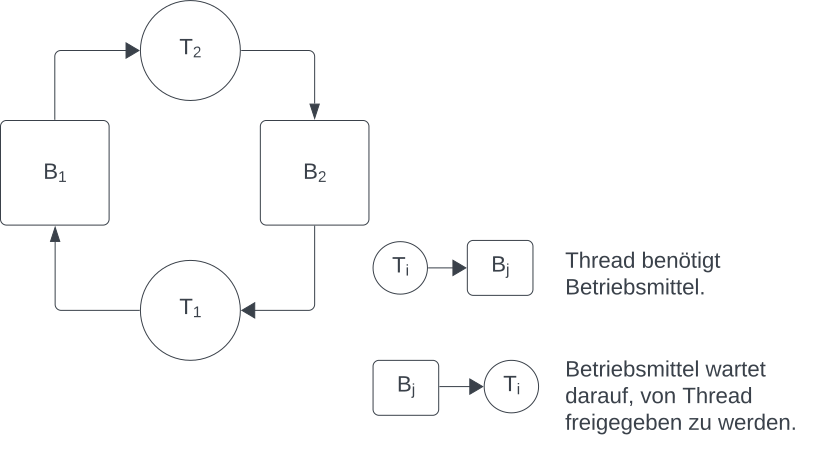
\includegraphics[scale=0.25]{chapters/3/img/cyclic}
            \caption{Betriebsmittelgraph. Quelle: in Anlehnung an \cite[192, Bild 3.9]{Oec22}}
            \label{fig:cyclic}
        \end{figure}
    \end{itemize}
\end{enumerate}


\section{Vermeidung von Verklemmungen}

Wenn eine der im vorherigen Abschnitt~\ref{sec:deadlockreason} genannten Bedingungen nicht gilt, kann keine Verklemmung vorliegen.\\

\noindent
In vielen Fällen ist \textbf{gegenseitiger Ausschluss} notwendig, weshalb Punkt 1 nicht abgeändert werden kann.\\

\noindent
Realisierung von \textbf{Betriebsmittelentzug} (Punkt 2) ist möglich, aber aufwändig.\\

\noindent
Gegenmaßnahmen ergeben sich aus den Bedingungen in Punkt 3 und 4\footnote{
vgl. im folgenden \cite[192 f.]{Oec22}.
}.\\

\begin{enumerate}
    \item Ein Thread darf nur Betriebsmittel anfordern, wenn er selbst keine Betriebsmittel besitzt (Nichterfüllung Punkt 3)
    \item Anforderung von Betriebsmitteln in einer bestimmten Reihenfolge, so dass garantiert werden kann, dass keine zyklischen Wartebedingungen entstehen (Nichterfüllung Punkt 4)
    \item Ein Trhead $t_1$ darf auf ein Betriebsmittel, dass $t_2$ gerade benutzt, nur warten, wenn bestimmte Beziehungen zwischen $t_1$ und $t_2$ gelten, damit keine zyklischen Wartebeziehungen entstehen (Nichterfüllung Punkt 4)
    \item Eine Bedarfsanalyse untersucht bei der Anforderung von Betriebsmitteln, ob es im worst-case bei Erfüllung der Anforderung zu Verklemmungen kommen kann - wenn selbst im worst-case keine Verklemmung entstehen kann, wird die Anforderung erfüllt (Nichterfüllung Punkt 4)
\end{enumerate}\\

\noindent
Realisierung mit Hilfe eines \textbf{ResourceManagers}, der alle Betriebsmittel kennt.\\

\noindent
Threads fragen ResourceManager an, der die Betriebsmittel dann zuweist.\\

\noindent
Anfordern von Betriebsmittel auf einen Schlag (s. \textbf{Semaphorgruppe}), damit es zu keener Verklemmung kommen kann (s. \textbf{Philosophenproblem}).\\

\noindent
Betriebsmittel gemäß einer vorgegebenen Reihenfolge anfordern, damit keine Verklemmungen entstehen können.\\
Bspw. durch Nummerierung der Betriebsmittel in \underline{aufsteigender Reihenfolge}, so dass ein Thread nur Betriebsmittel des Typs $s$ anfordern darf, wenn er keine Betriebsmittel des Typs $s$ oder $t > s$ hält\footnote{
    dann werden ihm nur Betriebsmittel vom Typ $t < s$ zugeteilt.
}).\\
Umsetzung beim Philosophenproblem: Alle Philosophen bis auf einen fordern zunächst links, dann rechts an, und einer in umgekehrter Richtung (man erhält dann immer eine verklemmungsfreie Lösung, vgl.~\cite[197]{Oec22}).\\

\noindent
Anforderung von Betriebsmitteln mit Bedarfsanalyse (\textbf{Bankier-Algorithmus}); Überprüfen der Anforderungen in Hinsicht auf sichere/unsichere Belegzustände, nur zuteilen von Betriebsmitteln, wenn sichere Belegzustände garantiert werden können.


\subsection{Zusammenfassung}
Eine \textbf{Verklemmung} ist eingetreten, wenn es einen Zyklus von Threads gibt, so dass ein Thread auf ein Betriebsmittel wartet, welches der im Zyklus folgende Thread besitzt.\\

\noindent
\textbf{Betriebsmittel}: Objekte, deren Zugriff mittels \code{synchronized}, \textbf{Semaphore} oder \textbf{Locks} synchronisiert werden.\\

\noindent
Voraussetzung für Verklemmungen sind, dass Betriebsmittel nur unter gegenseitigem Ausschluss nutzbar sind, einem Thread nicht entzogen werden können, und dass ein Thread bereits Betriebsmittel hält und weitere anfordert.\\

\noindent
Zur Vermeidung von Verklemmungen bieten sich verschiedene Strategien an, {bspw.} Anfordern der Betriebsmittel auf einen Schlag, in deiner bestimmten Reihenfolge oder Durchführung einer Bedarfsanalyse vor der Zuteilung, {bspw.} mithilfe des Bankier-Algorithms.
